\section{Introduction}
\label{introduction}

Real-time control of physical systems, like autonomous robots, raises a number of timing and control-related issues at the interface between the controller that's providing the actuation and the estimator that's providing periodic state estimates to the controller.
Some of these issues have to do with the inaccuracies introduced by the software implementation of both controller and estimator on a given hardware platform.
Specifically, controllers are typically designed to accomplish the functional goals of the system under simplifying assumptions on the quality of the state estimate (e.g., no or fixed error), the estimation delay (e.g., no or fixed delay), and the actuation jitter (e.g., no jitter).
Conversely, estimation algorithms are typically designed without regard to how their estimates will be used and under what operating conditions.
In particular, an estimator will often \emph{run to completion}: that is, its stopping criteria are designed to provide the best estimate, regardless of runtime or energy consumption.
The problem addressed here is that as the real-time requirements on the closed-loop system become more stringent, this separation in the design and execution of controller and estimator can lead to degraded performance, as will be shown in Example \ref{motivatingExample}.
The goal of this paper is to present a rigorous framework for the joint design of the controller and estimator, in which the estimator explicitly presents a range of execution time/estimate error operating modes, and the controller switches between these modes in real-time to maintain control performance and reduce energy consumption.
%Note that the first effect (estimate error) is due to the estimation algorithm itself regardless of implementation, whereas the last two effects (delay and jitter) have to do with the software implementation and its characteristics on the hardware platform.

%For example, the Computer Vision-based estimator we introduce in Section \ref{delayErrorCurve} uses a corner detector.
%In general, the corner detector will find the largest number of corners in a frame for best performance. 
Typical design practice determines the Worst-Case Execution Time (WCET) of the estimation task, and engineers the system to satisfy deadlines under WCET conditions.
However, the actual execution time of such estimators is heavily dependent on the actual data being processed. 
So WCET considerations, whether computed online or offline, produce a conservative design.
Moreover, classical timing analysis does not guarantee \emph{functional} correctness of the closed-loop system.
In addition, the best estimate is not always needed:
sometimes a lower quality estimate, obtained with a smaller energy cost, is sufficient to achieve the control objectives.
Finally, when obtaining better estimates requires longer runtimes of the estimation task, it may actually be detrimental to ask for the best estimate.
For example, when the computational resources are overloaded, there may be a need to spend less time computing a state estimate. 

\begin{figure}[t]
	\centering
	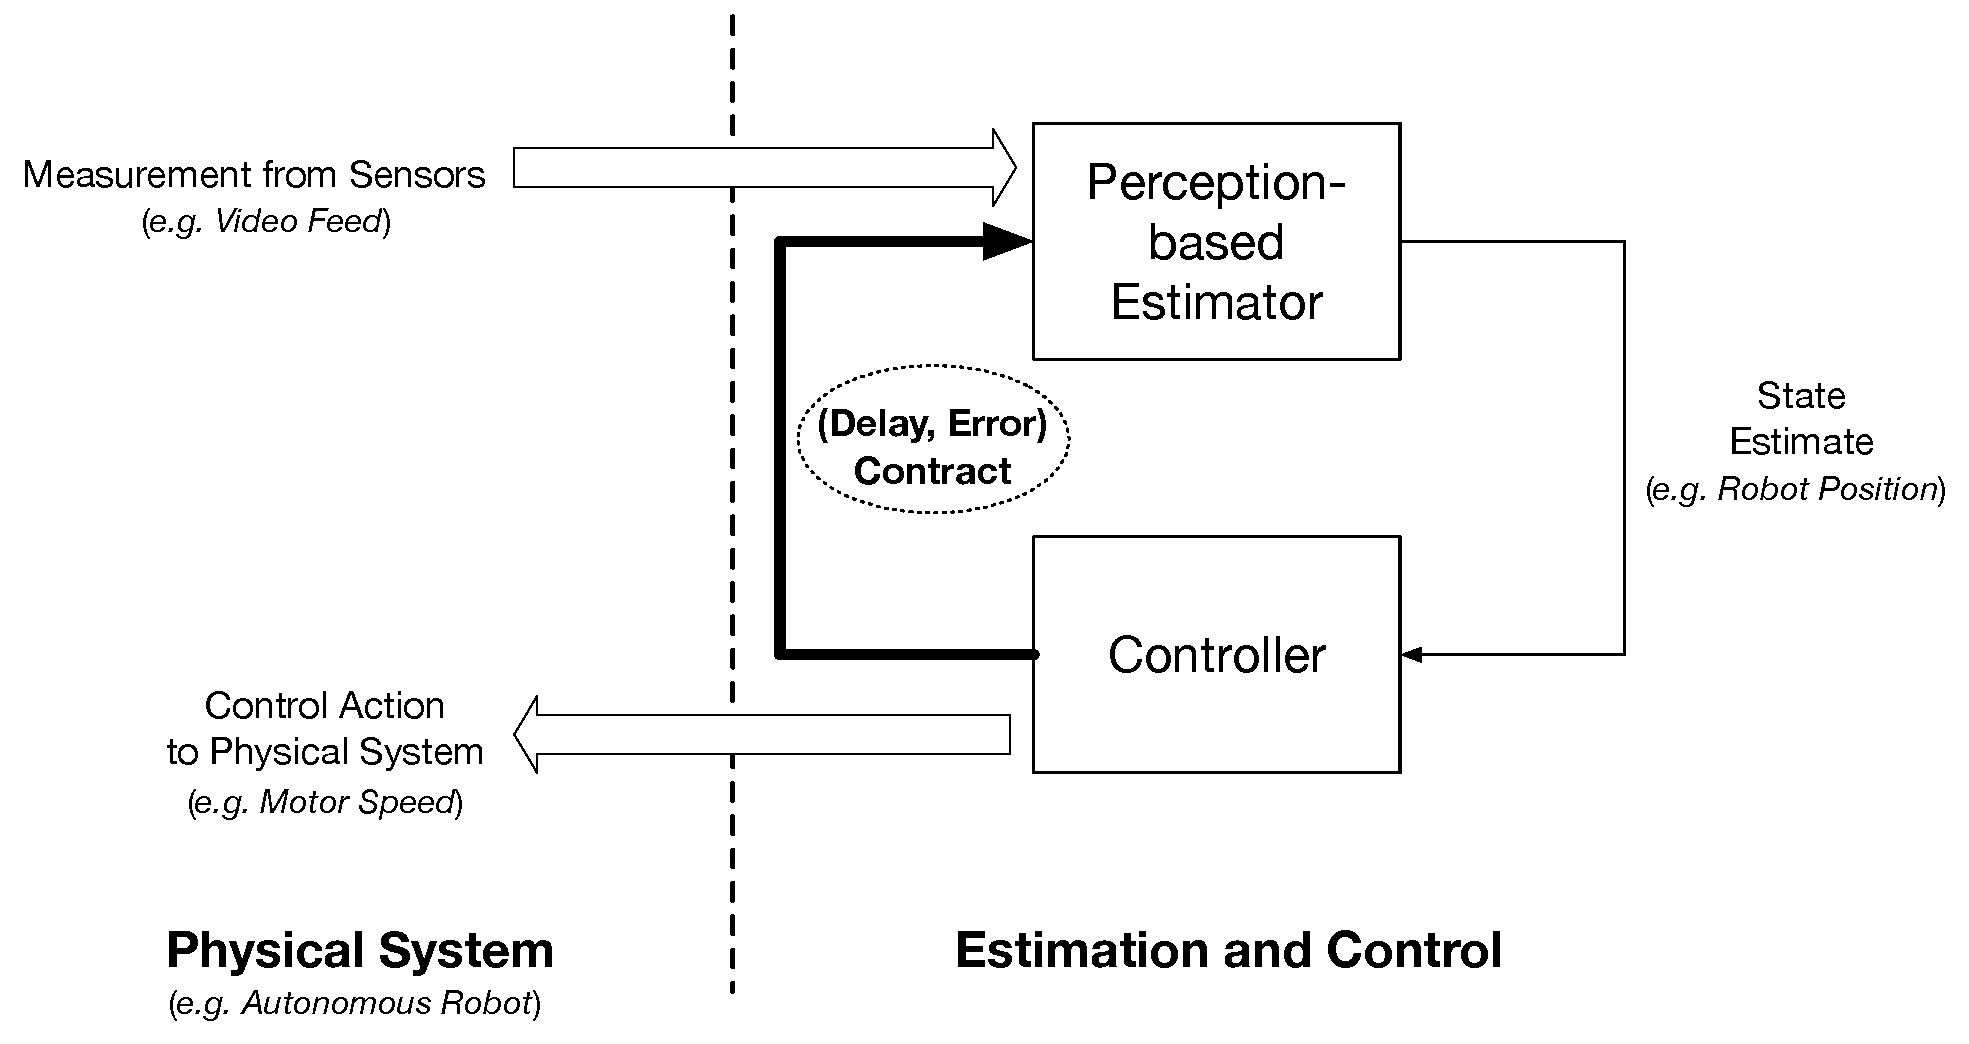
\includegraphics[scale=0.3]{figures/omnigraffle_figures/high_level_figure.pdf}
	\caption{Contract-based controller and estimator.}
	\label{fig:codesignedCE}
\end{figure}

\subsection{Motivating Example}
\label{motivatingExample}

As a motivating example, we consider the problem of autonomous flight of a hexarotor along a pre-defined pattern.
A hexarotor is a flying robot with six rotating blades.[???]
It carries a downward facing camera that sees salient features of the environment. 
See Fig.~\ref{fig:hexarotor}.
\begin{figure}[t]
	\centering
	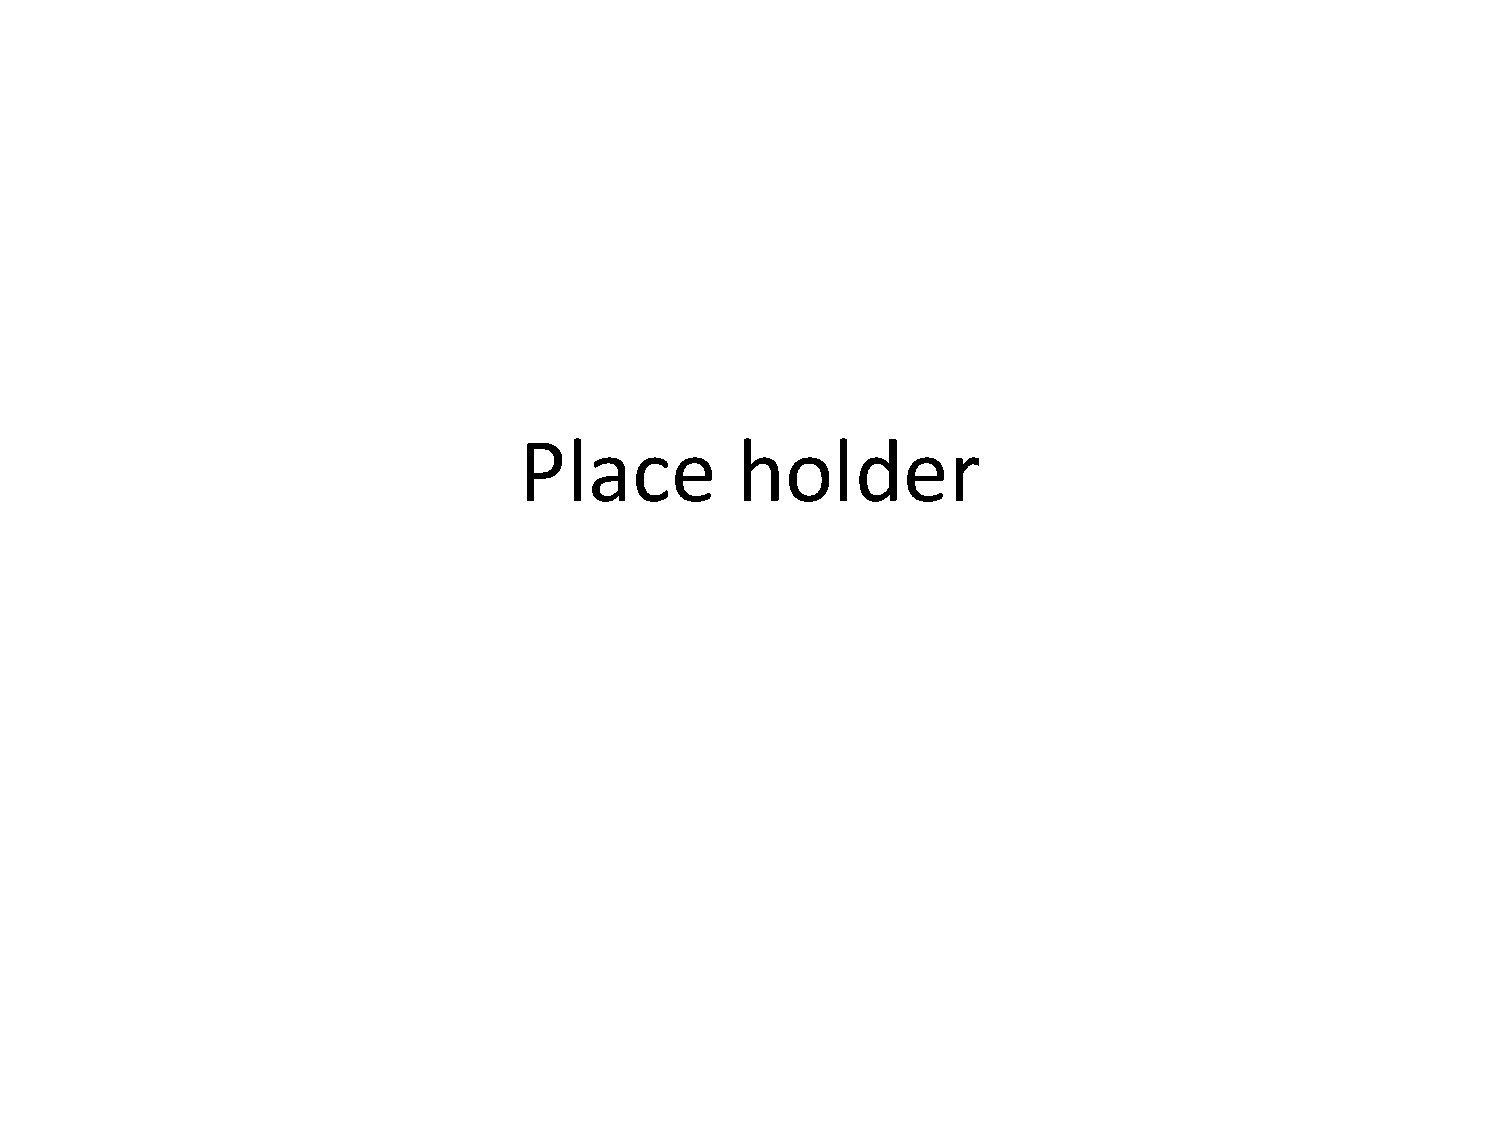
\includegraphics[width=0.7\linewidth]{figures/placeHolder}
	\caption{Hexarotor flying over synthetic features}
	\label{fig:hexarotor}
\end{figure}
These are detected by an on-board corner detector, and tracked across frames.
This allows the robot to estimate its own position in the world.
After each frame is acquired, the corner detector requires some computation time before producing its results, which are used in self-localization.
Thus the control command which uses this estimate is delayed by the time necessary to run the estimation task to completion.
This is illustrated in Fig.~\ref{fig:senseActuateDelay}.
\begin{figure}[t]
	\centering
	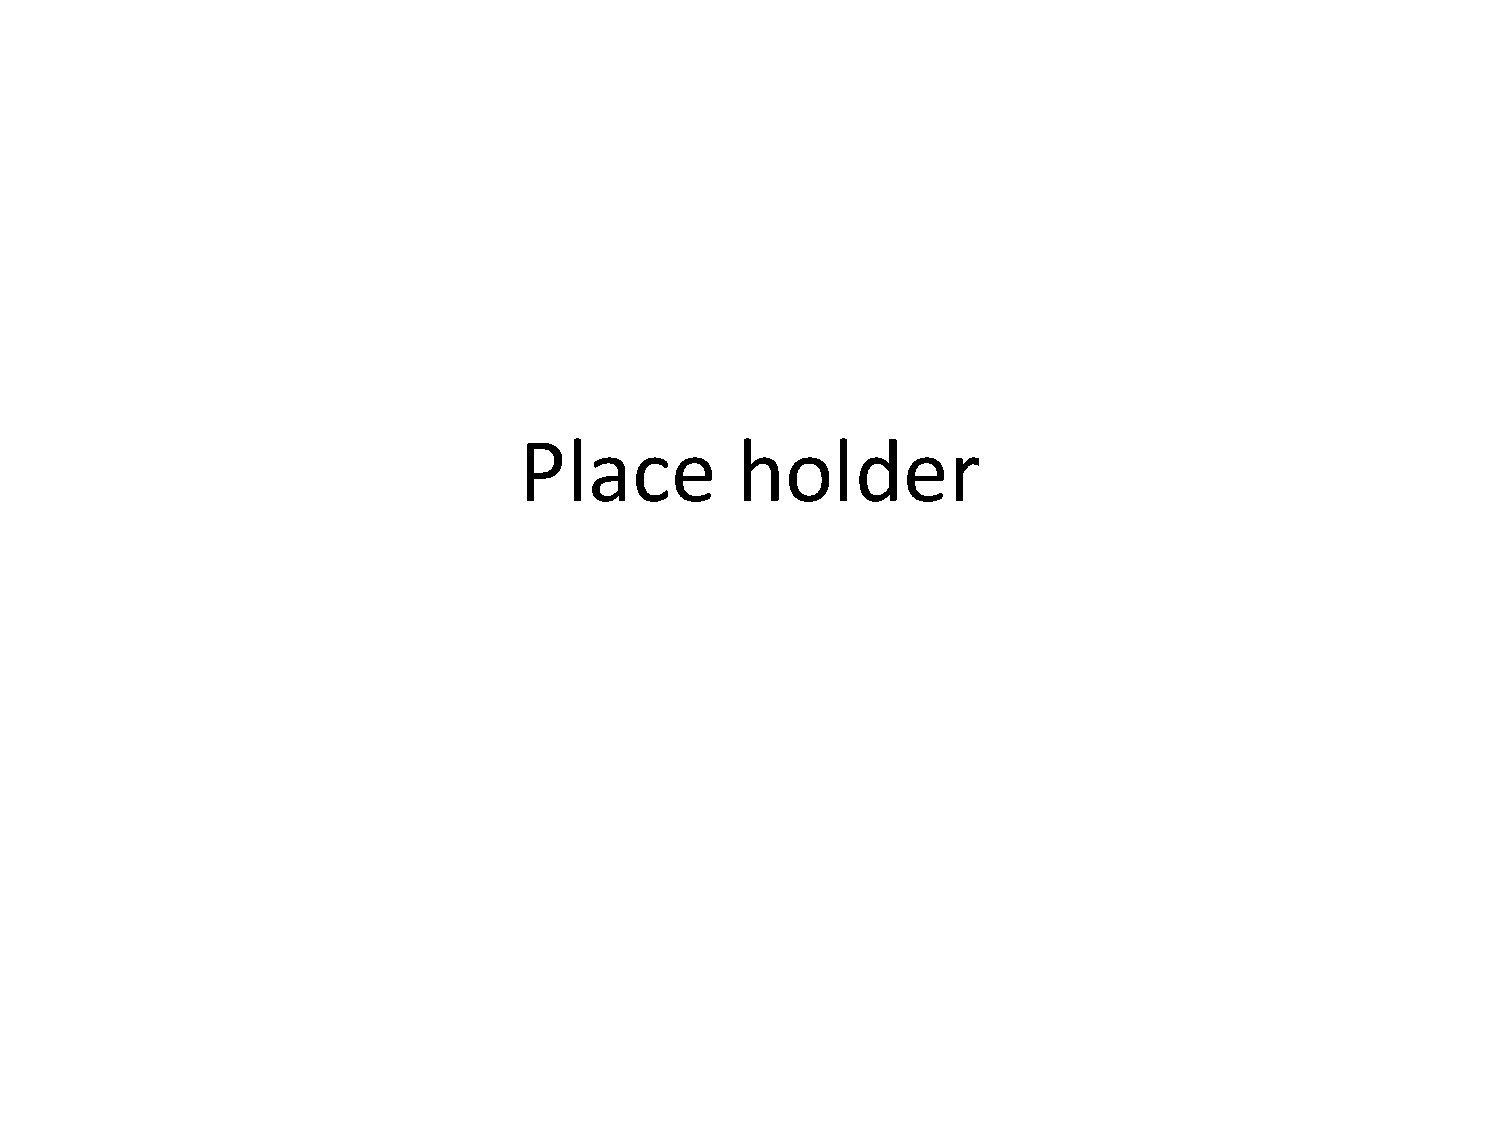
\includegraphics[width=0.7\linewidth]{figures/placeHolder}
	\caption{Sense-Estimate-Actuate cycle. The estimation task always runs to completion.}
	\label{fig:senseActuateDelay}
\end{figure}
The robot has a high-level controller which determines the desired pitch and roll angles, and desired rotor thrust. 
In this implementation, we use a Model Predictive Controller (MPC) [???].
As the robot is commanded to fly the pattern faster and faster, the estimator delay affects the control performance more.
\todo[inline]{Pending experiemental confirmation about the effect of speed of flight on control performance }
The control performance, as measured by a function that factors in the error in following the flight path and the cost of control, is shown in Fig.~\ref{fig:degradingPerformance}.
(The details of this cost function are given in Section \ref{formulation}).
\begin{figure}[t]
	\centering
	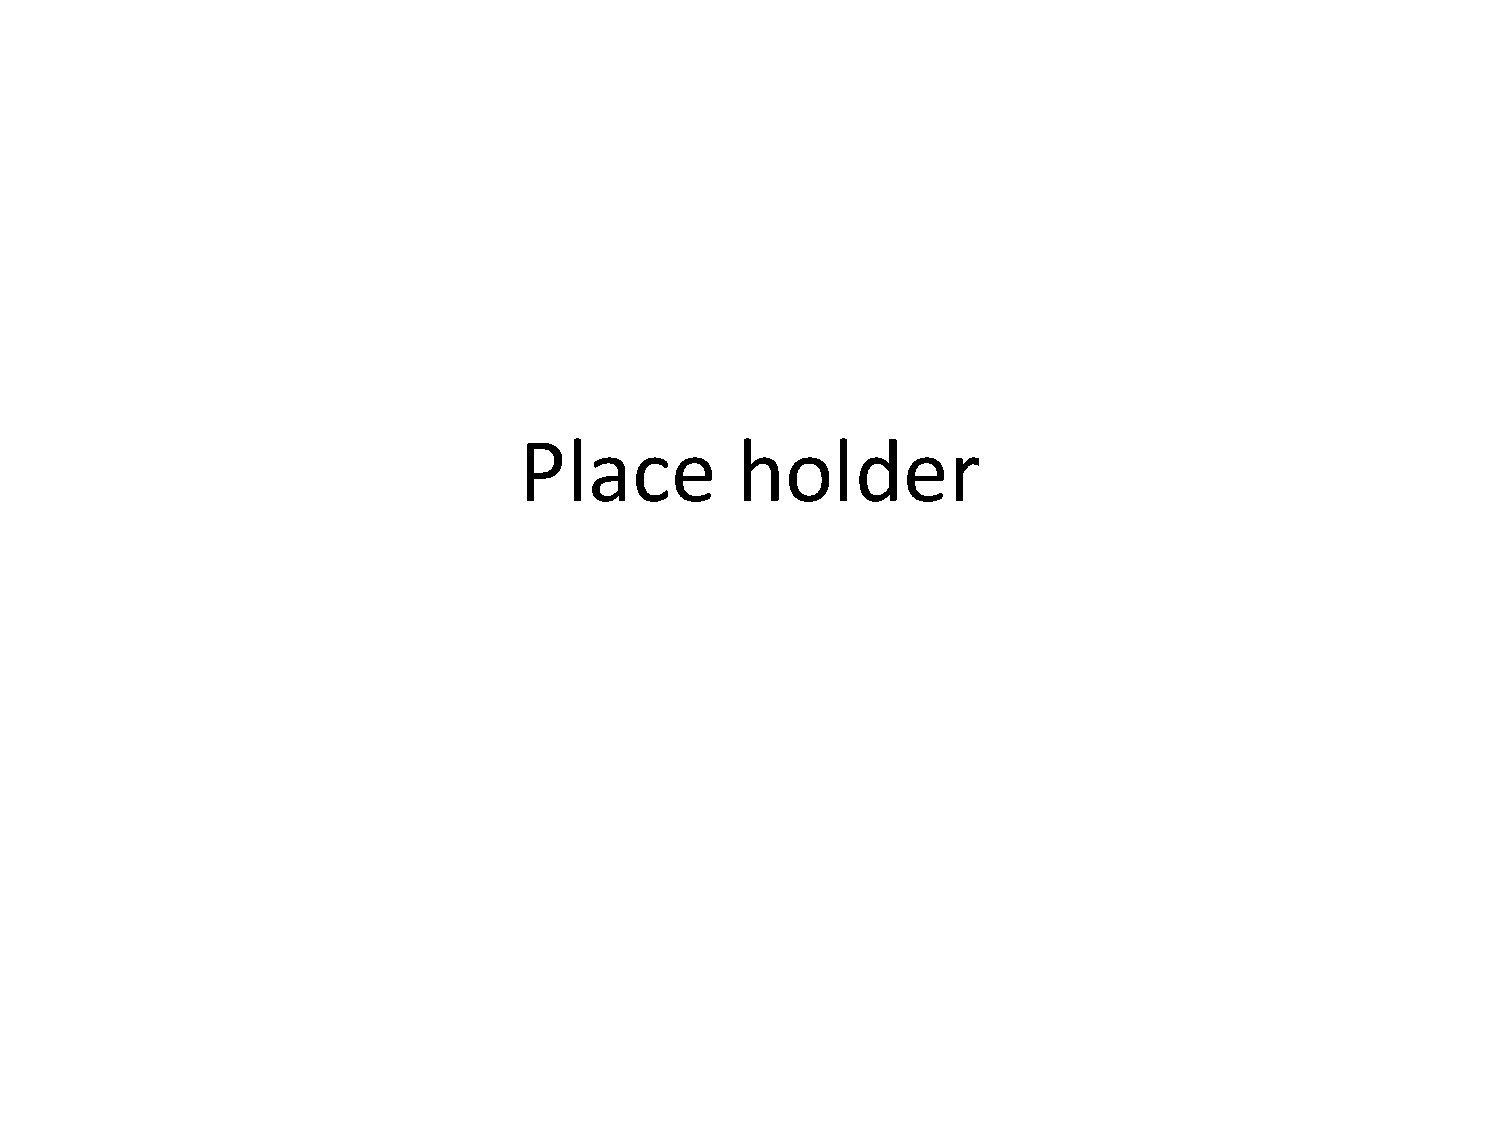
\includegraphics[width=0.7\linewidth]{figures/placeHolder}
	\caption{Degrading performance as the control objectives become more stringent.}
	\label{fig:degradingPerformance}
\end{figure}
Running an estimation task with a fixed smaller delay but larger estimation error does not necessarily solve the problem of degraded performance, as shown in Fig.~\ref{fig:degradingPerformanceSmallDelta}.
\begin{figure}[t]
	\centering
	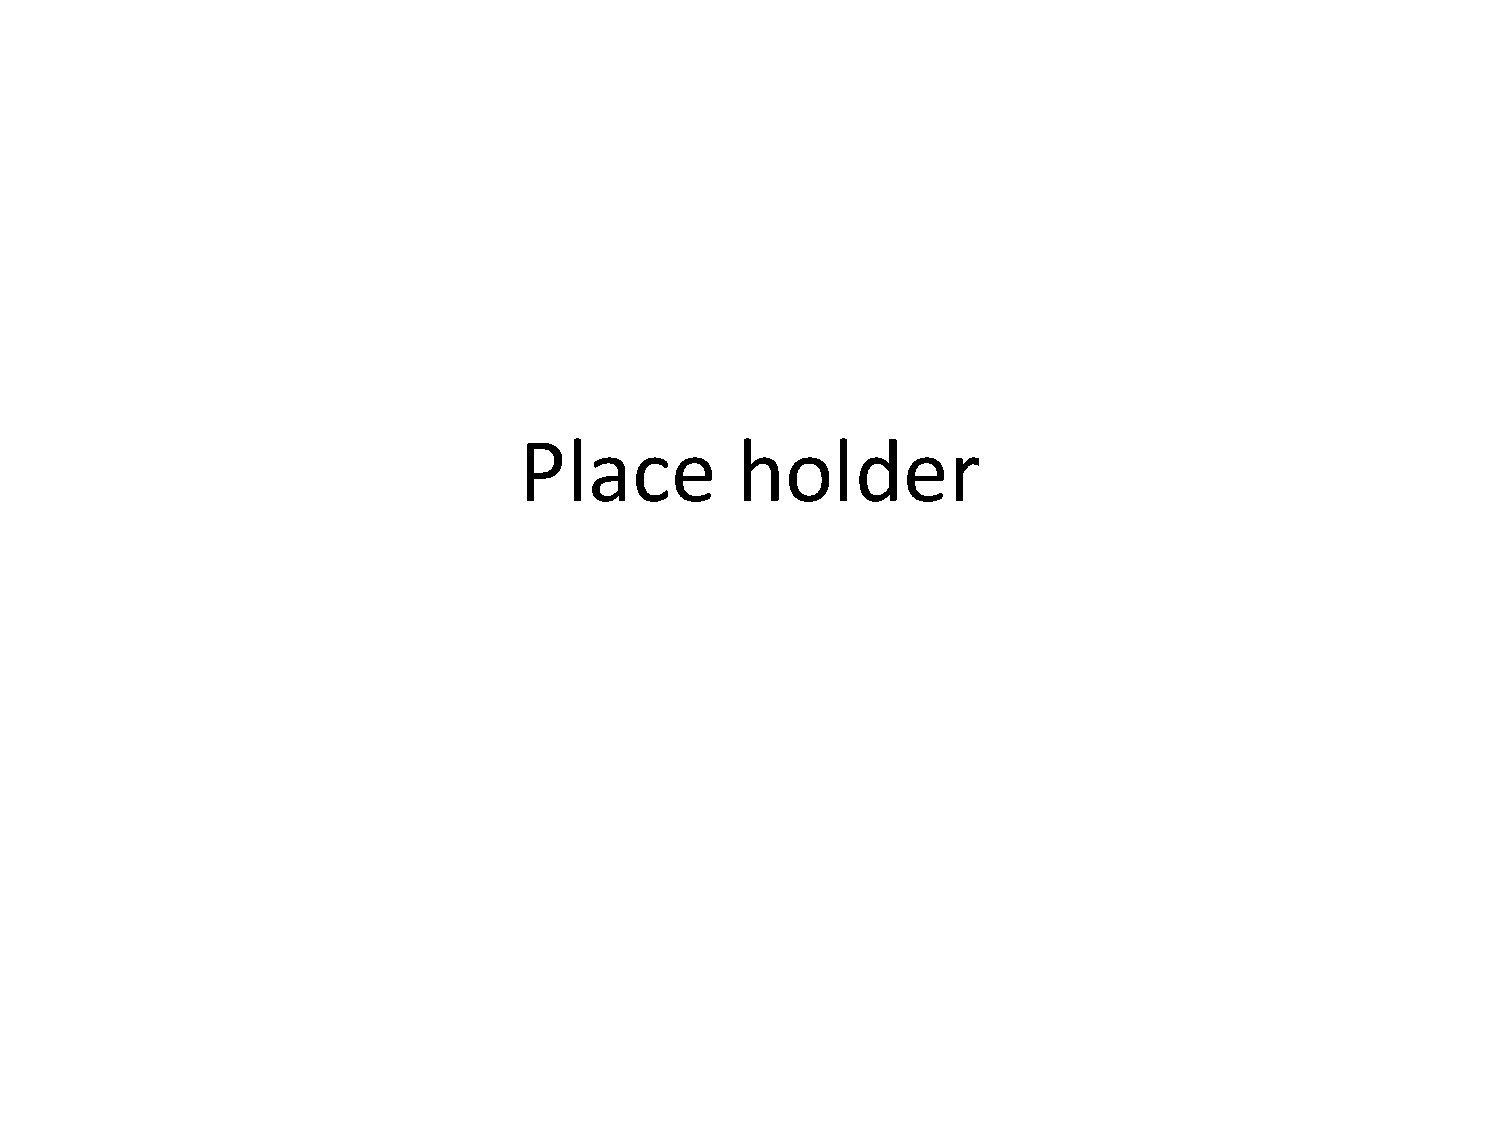
\includegraphics[width=0.7\linewidth]{figures/placeHolder}
	\caption{Degrading performance at a smaller fixed delay.}
	\label{fig:degradingPerformanceSmallDelta}
\end{figure}

Therefore, there is a need to rigorously quantify the trade-off between computation time and estimation error, then exploit that trade-off intelligently to achieve the best control performance under the problem constraints.
Rather than always run the estimation task to completion, it is useful to have several estimation tasks with varying utilities (i.e., varying delay/error trade-offs).
These can then be used at runtime to satisfy the control objectives.


In this work, we develop the above remarks into a \emph{co-design framework} for a real-time control systems, where the controller and estimator communicate via \emph{contracts}.
A contract is a guarantee requested by the controller, and fulfilled by the estimator, that the latter can provide an estimate with a certain maximum error $\sAccu$, and within a certain deadline $\sDelay$.
Both the deadline and the error bound are part of the contract.
Using these contracts, we show how the controller can throttle the execution time of the estimation task to preserve good performance and to reduce energy consumption.
Our work focuses on estimators that incorporate computationally intensive Computer Vision (CV) algorithms, such as those used in autonomous robot navigation. 
We refer to these as \emph{perception-based estimators}.
Our experiments validate that the execution time of these algorithms is significant and far exceeds the computation time of the control software, and can have an effect on control performance.

Fig.~\ref{fig:codesignedCE} presents the proposed structure of contract-based estimation and control.
It shows a traditional feedback loop incorporating estimator, controller and the physical system, augmented with the (Delay, Error) contract between controller and estimator.
This contract forms the basis of the proposed approach.

\textbf{Summary of contributions}.
We present a contract-based framework for the co-design of real-time controller and estimator algorithms, consisting of:
\begin{itemize}
	\item a well-defined interface between control and estimation, in the form of operating modes or \emph{contracts} on the accuracy and delay provided by the estimator (Section \ref{sec:codesign}),
	\item a controller design that can vary the accuracy and delay of the estimation to achieve control objectives at a lower energy cost (Sections \ref{controlProblem}, \ref{robustMPC}), and
	\item a general procedure to compose run-to-completion estimation algorithms into a contract-based estimator (Section \ref{delayErrorCurve}).
	\item We illustrate our approach on an autonomous flying robot (shown in Fig.~\ref{fig:nanohex}) and demonstrate performance and energy gains using our approach over a classical controller (Section \ref{sec:experiments}).
\end{itemize}
\begin{figure}[t]
	\centering
	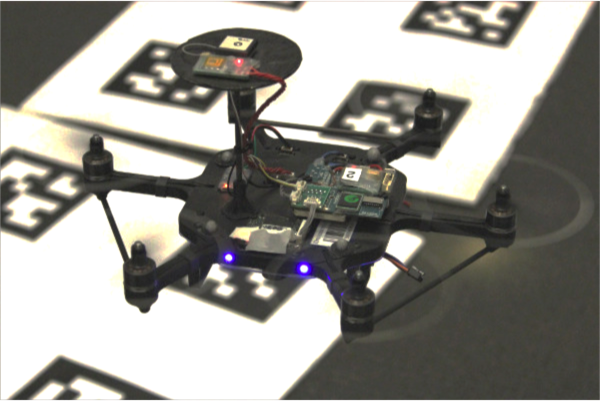
\includegraphics[width=0.7\linewidth]{figures/nanohex2}
	\caption{Autonomous hexrotor with downward-facing camera flying over synthetic features.}
	\label{fig:nanohex}
\end{figure}
\begin{figure*}[t]
	\centering
	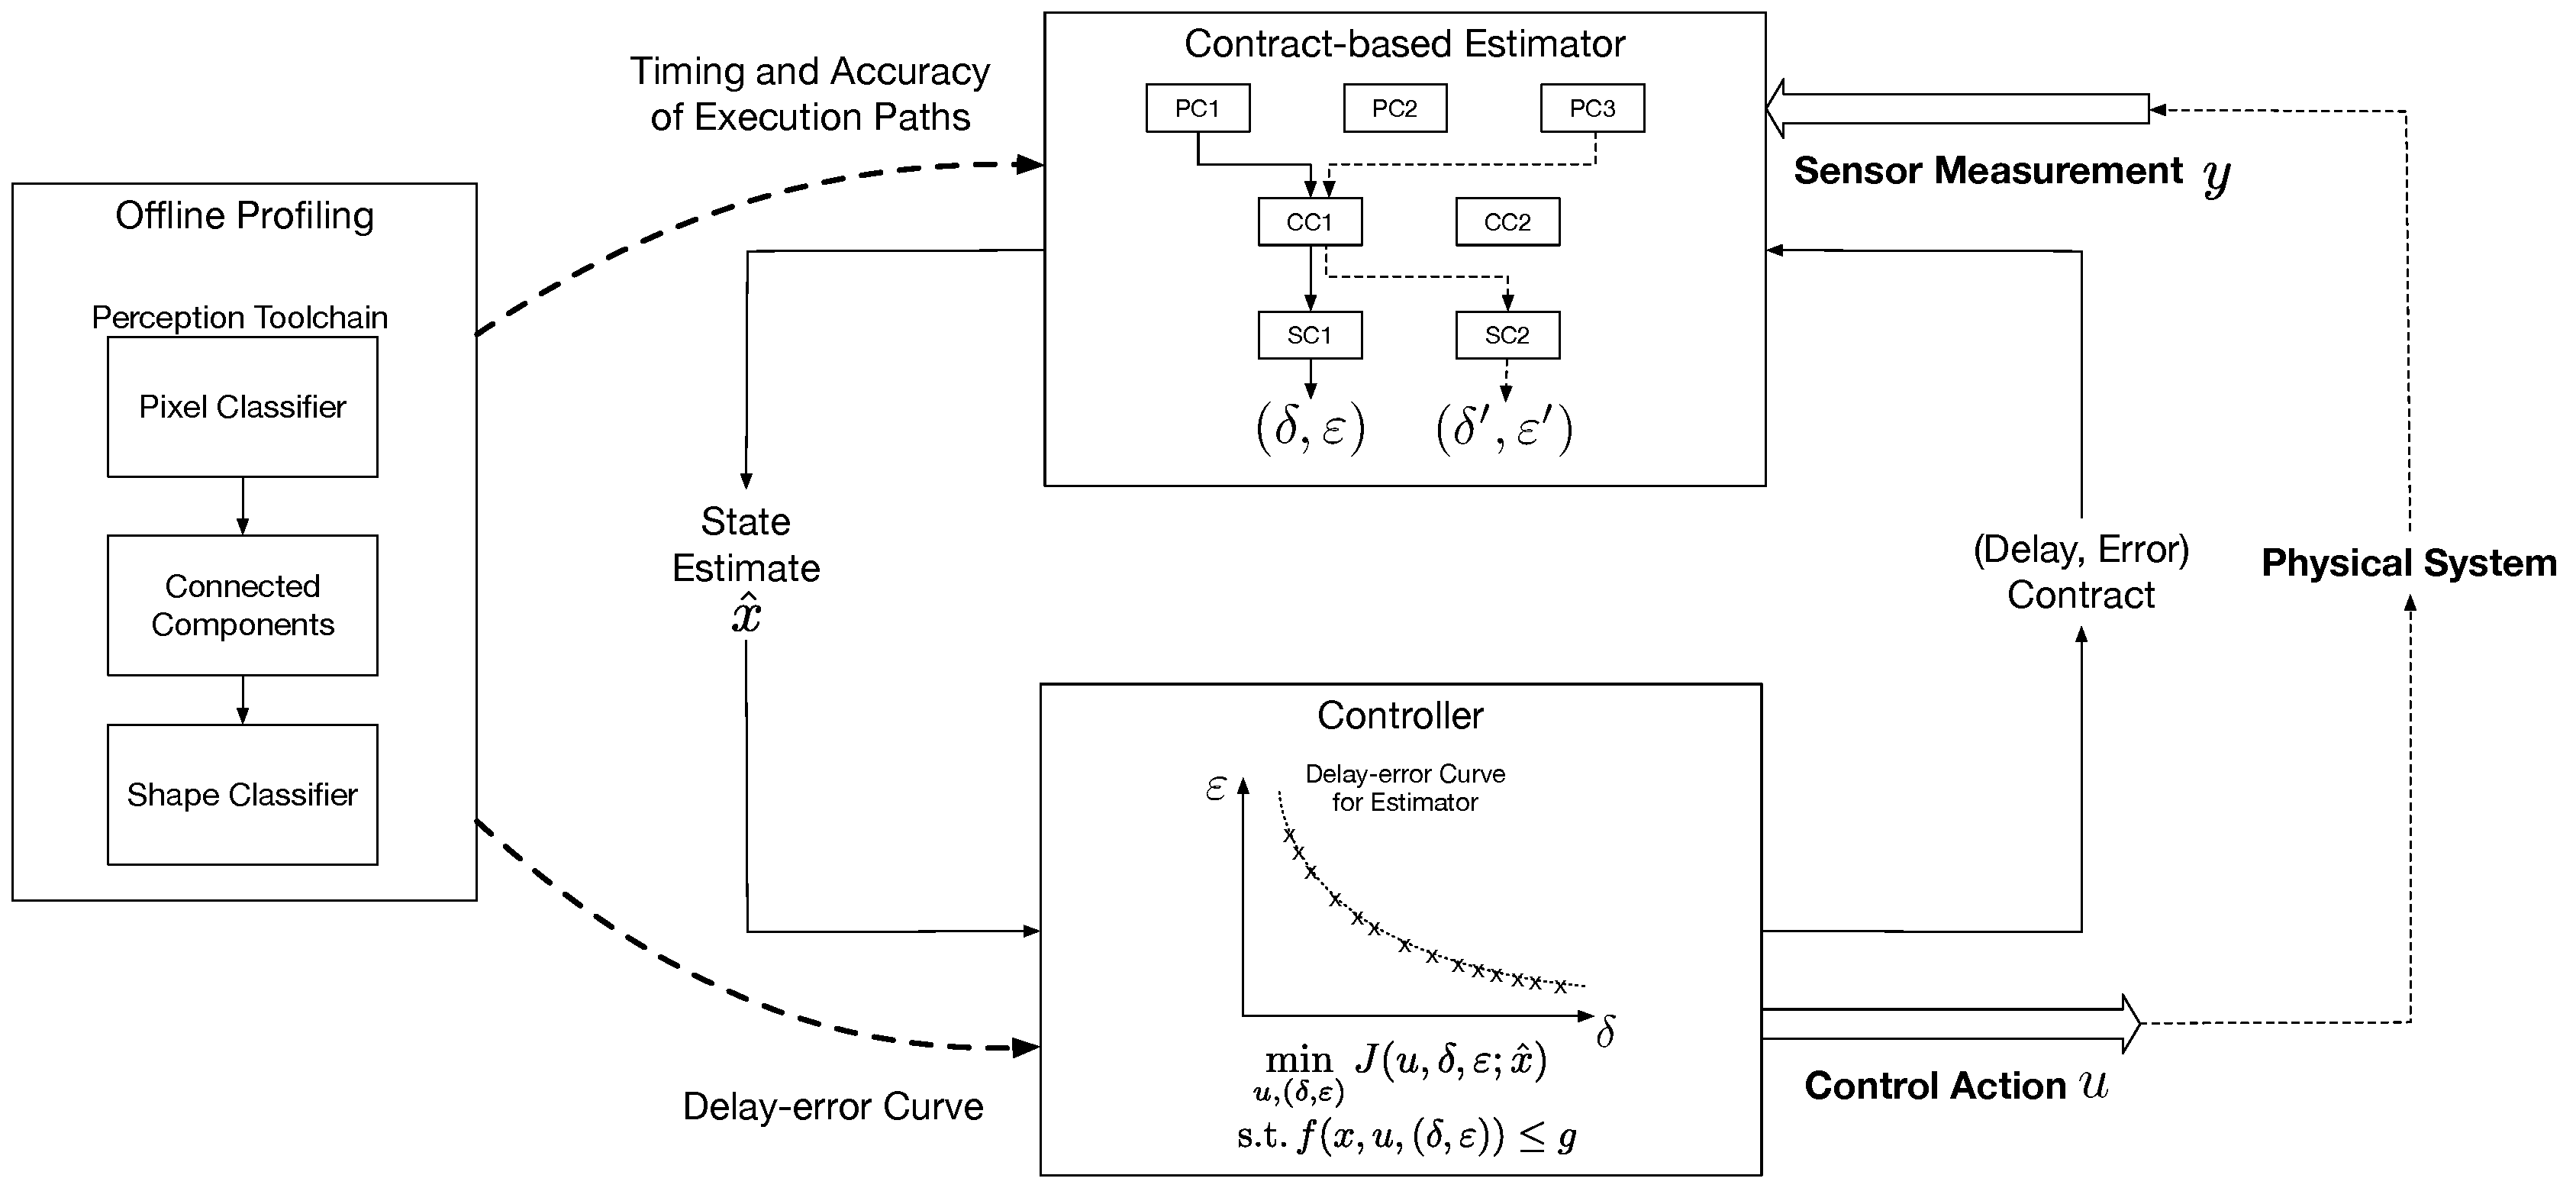
\includegraphics[width=0.9\textwidth]{figures/omnigraffle_figures/process_figure2}
	\caption{Contract-based estimator and controller}
	\label{fig:fullcodesignedCE}
\end{figure*}